%! TeX root = ../main.tex

\chapter{Numerical methods}%
\label{ch:numerical-methods}

The goal of this chapter is to explain the numerical implementation of our
impurity solver and subsequent DMFT self-consistency loop.
Most ideas are taken from~\cite{Lu2014, Lu2019, Kugler2022, Zacinskis2025}.

The main problem in quantum many-body physics the size of
the associated Hilbert space~\cite{Brass2021}.
In principle there are infinitely many states an electron can occupy.
One method to calculate models on a computer is therefore to discretize the space
by choosing a finite number $i\in\{1,\ldots,n\}$ of one-particle wave functions $\{\ket{\phi_i}\}$
with energies $\epsilon_i$.
They can be combined to create Slater determinants
\begin{equation}
    \ket{\alpha} = \prod_{i\sigma} \left(c^\dag_{i\sigma}\right)^n \ket{0},
    \quad
    n\in\{0,1\},
\end{equation}
which allows us to write wave functions as linear combinations
\begin{equation}
    \ket{\psi} = \sum_j \alpha_j \ket{\alpha_j}.
\end{equation}

As each site has four possible states\footnote{
    They are $\ket{0}$, $\ket{\uparrow}$, $\ket{\downarrow}$, and $\ket{\uparrow\downarrow}$.
}
the dimension of the Hilbert space grows as $4^n$ limiting exact diagonalization (ED)
to $\bigO{10}$ sites.
To further reduce the dimensionality of our space,
we can employ so-called \emph{quantum numbers}~\cite{Wallerberger2022}:
We look at symmetries of our Hamiltonian which allows us to decompose it into blocks
with no overlaps between those.
E.g., we introduce the number operator $N = \sum_{i\sigma} c^\dag_{i\sigma} c^{\pdag}_{i\sigma}$
and if our Hamiltonian conserves it $[H, N] = 0$,
we know that $H$ and $N$ share a common basis.
Thus, we can decompose our Hamiltonian into blocks of $p\in\{0, \ldots, 2n\}$ particles
where the dimensionality of each block is given by
\begin{equation}
    \binom{2n}{p}.
\end{equation}
As our Hamiltonian is SU(2) symmetric, % chktex 36
we can split it into blocks of fixed $N_\uparrow$ and $N_\downarrow$
further reducing the dimensionality to
\begin{equation}
    \binom{n}{p_\uparrow} \binom{n}{p_\downarrow}.
\end{equation}
For the half-filled block where $p_\sigma = n/2$ its asymptotic behavior is
\begin{equation}
    \binom{n}{n/2} \binom{n}{n/2}
    \approx
    \frac{2}{\muppi}\frac{4^n}{n},
\end{equation}
which for $n=140$ sites is approximately $\num{9e81}$
exceeding the number of protons in the observable universe $\bigO{\num{e80}}$. % Eddington number

\subsection{Natural impurity orbitals and restricted active space}%
\label{sec:NIO-RAS}

To mitigate this issue,
we take the same approach as~\cite{Lu2019}.
Instead of exploring the full Hilbert space of $n$ particles in an Anderson impurity model,
we consider only a very small subset.

In the first step,
the one particle basis $\{\ket{\phi_i}\}$ is optimized to the so-called
\emph{natural impurity orbitals} which
--- compared to the commonly used \emph{natural orbitals} in quantum chemistry ---
optimize only the bath basis while keeping the impurity unchanged\footnote{
    Otherwise,
    the Coulomb interaction (\zcref{eq:H-Anderson-interaction})
    is distributed onto many new sites and is not local anymore.
}.
This new geometry is shown in \zcref{fig:AIM-natural-impurity-orbitals}.
The untouched impurity $i$ is connected to a mirror site (labeled $m$) and two chains.
Following the convention of~\cite{Lu2014,Lu2019},
we call sites in the almost fully filled chain valence bath sites (labeled $v$),
and sites in the almost empty chain as conduction bath sites (labeled $c$).
Hopping between sites is again shown by lines.
\begin{figure}[ht]
    \centering
    %! TeX root = ../../main.tex

\begin{tikzpicture}[
        inner sep=1mm,
        node distance=4mm,
    ]
    % sites
    \node [impurity={0.5}] (impurity) {};
    \node [bath={0.5}] (mirror) [right=of impurity] {};
    \foreach \i [remember=\i as \lasti] in {1,...,6}
        {
            \ifnum\i=1
                \node [bath={0.85}] (v\i) [below=of mirror] {};
                \node [bath={0.15}] (c\i) [above=of mirror] {};
            \else
                \ifnum\i=2
                    \node [bath={0.9}] (v\i) [right=of v\lasti] {};
                    \node [bath={0.1}] (c\i) [right=of c\lasti] {};
                \else
                    \ifnum\i=4
                        \node [bath={1.0}] (v\i) [right=8mm of v\lasti] {};
                        \node [bath={0.0}] (c\i) [right=8mm of c\lasti] {};
                    \else
                        \node [bath={1.0}] (v\i) [right=of v\lasti] {};
                        \node [bath={0.0}] (c\i) [right=of c\lasti] {};
                    \fi
                \fi
            \fi
        }

    % labels (separate node for box fit below)
    \node (impuritylabel)[left=0mm of impurity] {$i$};
    \node (mirrorlabel)[right=0mm of mirror] {$m$};
    \node (v1label)[below=0mm of v1] {$v_1$};
    \node (v3label)[below=0mm of v3] {$v_{L\vphantom{+1}}$}; % phantom for bounding box size
    \node (v4label)[below=0mm of v4] {$v_{L+1}$};
    \node (c1label)[above=0mm of c1] {$c_1$};
    \node (c3label)[above=0mm of c3] {$c_{L\vphantom{+1}}$}; % phantom for bounding box size
    \node (c4label)[above=0mm of c4] {$c_{L+1}$};


    % connect sites
    \draw (impurity.east) to (mirror.west);
    \draw (impurity.south) to [out=270,in=180] (v1.west);
    \draw (impurity.north) to [out=90,in=180] (c1.west);
    \draw (mirror.south) to (v1.north);
    \draw (mirror.north) to (c1.south);
    \foreach \i [remember=\i as \lasti (initially 1)] in {2,...,6}
        {
            \draw (v\lasti.east) -- (v\i.west);
            \draw (c\lasti.east) -- (c\i.west);
        }

    % bounding box
    \node [
        draw,
        rectangle,
        rounded corners,
        line width=0.2pt,
        fit=(impuritylabel) (v3label) (c3label),
        label=left:$|\phi_I\rangle$,
    ] {};
    \node [
        draw,
        rectangle,
        rounded corners,
        line width=0.2pt,
        fit=(v4label) (v6) (c4label) (c6),
        label=right:$|\phi_{II}\rangle$,
    ] {};
\end{tikzpicture}

    \caption{
        Anderson impurity model in the natural orbital basis and
        subsequent separation of the wave function into two components
        $\ket{\psi_\mathrm{I}}$ and $\ket{\psi_\mathrm{II}}$ denoted by two boxes.
    }%
    \label{fig:AIM-natural-impurity-orbitals}
\end{figure}

This however, does not change the dimensionality of the Hilbert space.
To alleviate the scaling problem we employ the restricted active space (RAS) method,
which decomposes the wave function into two components
\begin{equation}
    \ket{\psi} = \ket{\psi_\mathrm{I}} \otimes \ket{\psi_\mathrm{II}}
\end{equation}
sketched in \zcref{fig:AIM-natural-impurity-orbitals}.
For $\ket{\psi_\mathrm{I}}$ we take all possible states into account.
This is feasible because we fix the parameter $L$
(the number of conduction and valence bath sites to be treated exactly)
to be very small compared to the number of bath sites $L \ll n$.

In $\ket{\psi_\mathrm{II}}$ which contains the remaining chain sites we neglect almost all
possible electron configurations.
In the simplest approximation (labeled $p=0$)
we enforce that all valence sites in $\ket{\psi_\mathrm{II}}$
are fully filled (denoted by $\ket{\mathbb{1}_v}$) while
conduction sites are completely empty (denoted by $\ket{\mathbb{0}_c}$).
The wave function can thus be written as
\begin{equation}
    \ket{\psi_\mathrm{II}} = \ket{\mathbb{1}_v} \otimes \ket{\mathbb{0}_c}.
\end{equation}

For $p=1$ we additionally to $p=0$ allow one electron or one hole excitation.
This creates possible states
\begin{subequations}
    \begin{align}
        \ket{\mathbb{1}_v}             & \otimes c^\dag_{k\sigma} \ket{\mathbb{0}_c}, \\
        v_{k\sigma} \ket{\mathbb{1}_v} & \otimes \ket{\mathbb{0}_c}.
    \end{align}
\end{subequations}

This can be further extended to $p=2$ which
(including all previous excitations)
contains electron-electron, electron-hole, and hole-hole excitations
\begin{subequations}
    \begin{align}
        \ket{\mathbb{1}_v}                           & \otimes c^\dag_{k\sigma} c^\dag_{k'\sigma'} \ket{\mathbb{0}_c}, \\
        v_{k\sigma} \ket{\mathbb{1}_v}               & \otimes c^\dag_{k'\sigma'} \ket{\mathbb{0}_c},                  \\
        v_{k\sigma} v_{k'\sigma'} \ket{\mathbb{1}_v} & \otimes \ket{\mathbb{0}_c}.
    \end{align}
\end{subequations}

Theoretically, one can continue this approach to higher and higher orders
with the limit of all excitations recovering the full Hilbert space
(including the exponential growth of the available configurations).
In this work we only implemented excitations up to $p=2$,
as higher $p$ are not numerically feasible for hundreds of bath sites.

\section{Lanczos algorithm}%
\label{sec:Lanczos-algorithm}

Even with RAS,
the Hilbert space is still too large decompose the Hamiltonian.
Therefore,
we use the Lanczos algorithm~\cite{Lanczos1950}
as it has some nice properties for our given problem.
First,
it converges fastest to extremal eigenvalues which
works very well for the ground state\footnote{
    Due to the variational principle it is the state with the lowest possible energy
    which is extreme.
}
and as DMFT is a low-energy theory we are not interested in states very far from it.
Secondly, it requires a hermitian matrix which our Hamiltonian is.
Lastly it works very well if our matrix is sparse which is the case for our geometry\footnote{
    As most of it is composed of two long chains,
    almost all hopping elements are zero.
}.
The method is based on a Krylov basis
\begin{equation}
    \mathcal{K}^M(H, \vec{q}) = \spn\{\vec{q}, H\vec{q}, H^2\vec{q}, \ldots, H^{M-1}\vec{q}\}
\end{equation}
for a given vector $\vec{q}$.
Typically, the value $M$ is very small compared to the matrix size.
Instead of a simple power iteration, the Lanczos algorithm is described by the
following recurrence relation
\begin{equation}
    b_j\vec{q}_{j+1} = H\vec{q}_j - a_j\vec{q}_j - b_{j-1}\vec{q}_{j-1}
    \label{eq:Lanczos-recurrence}
\end{equation}
with a normalized starting vector $\vec{q}_1$ and $\vec{q}_0 = \vec{0}$.
The coefficients are chosen such that each Lanczos vector $\vec{q}_j$ is orthonormal to each other
\begin{equation}
    a_j = \vec{q}_j^\dag H \vec{q}_j,
    \qquad
    b_j = \vec{q}_{j+1}^\dag H \vec{q}_j.
\end{equation}
For numerical stability~\cite{Paige1972, Paige1976}
we instead calculate the coefficients as
\begin{equation}
    a_j = \vec{q}_j^\dag(H \vec{q}_j - \beta_{j-1}\vec{q}_{j-1}),
    \qquad
    b_j = \norm{H\vec{q}_j - \alpha\vec{q}_j -  \beta_{j-1}\vec{q}_{j-1}}.
\end{equation}
From this relation we can create the tridiagonal matrix
\begin{equation}
    T
    =
    \begin{pmatrix}
        a_1 & b_1 &        &         &         \\
        b_1 & a_2 & b_2    &         &         \\
            & b_2 & a_3    & \ddots  &         \\
            &     & \ddots & \ddots  & b_{M-1} \\
            &     &        & b_{M-1} & a_M
    \end{pmatrix},
    \label{eq:tridiagonal-scalar}
\end{equation}
and matrix collecting all Lanczos vectors
\begin{equation}
    Q = (\vec{q}_1, \vec{q}_2, \ldots, \vec{q}_M).
\end{equation}
Rewriting \zcref{eq:Lanczos-recurrence} in matrix form and rearranging results in $T = Q^\dag H Q$,
which means that $T$ is the orthogonal projection of $H$ onto
the subspace $\mathcal{K}^M(H, \vec{q}_1)$~\cite{Cullum1985}.

\subsection{Block variant}

Instead of calculating only one vector $\vec{q}_j$ in each step,
one can calculate $p$ vectors simultaneously.
We define
\begin{equation}
    Q_1 = (\vec{q}_1^{(1)}, \vec{q}_1^{(2)}, \ldots, \vec{q}_1^{(p)})
\end{equation}
to be an $n\times p$ orthonormal block of starting vectors
and $Q_0 = \mathbb{0}_{n\times q}$.
Then the recurrence relation (\zcref{eq:Lanczos-recurrence}) can be rewritten as
\begin{equation}
    Q_{j+1} B_j = H Q_j - Q_j A_j - Q_{j-1} B_{j-1}^\dag,
    \label{eq:block-Lanczos-recurrence}
\end{equation}
with $A_j$, $B_j$ matrices of size $p\times p$ chosen such that each block $Q_j$ is orthonormal
to each other.
The block tridiagonal matrix of size $Mp\times Mp$ is written as
\begin{equation}
    T
    =
    \begin{pmatrix}
        A_1 & B_1^\dag &          &         &              \\
        B_1 & A_2      & B_2^\dag &         &              \\
            & B_2      & A_3      & \ddots  &              \\
            &          & \ddots   & \ddots  & B_{M-1}^\dag \\
            &          &          & B_{M-1} & A_M
    \end{pmatrix}.
    \label{eq:tridiagonal-block}
\end{equation}
For the calculation for $B_j$ one needs to orthonormalize
\begin{equation}
    \tilde Q_{j+1} = H Q_j - Q_j A_j - Q_{j-1} B_{j-1}^\dag,
\end{equation}
which is not unique.
For instance, a QR decomposition $Q_{j+1} B_j = \tilde Q_{j+1}$
results in an upper triangular matrix $B_j$
which gives $T$ a compactly banded structure~\cite{Cullum1985, Golub2013}.
In our work however, we use symmetric Löwdin orthonormalization~\cite{Lowdin1950, Brass2021}
which is based on the singular value decomposition
$\tilde Q_{j+1} = U \Sigma V^\dag$.
We define the overlap matrix as
\begin{equation}
    S \coloneqq \tilde Q_{j+1}^\dag \tilde Q_{j+1} = V \Sigma^2 V^\dag
\end{equation}
and its roots as
\begin{equation}
    S^{1/2} = V \Sigma V^\dag,
    \qquad
    S^{-1/2} = V \Sigma^{-1} V^\dag.
\end{equation}
The resulting vectors are then
\begin{align}
    Q_{j+1} & = \tilde Q_{j+1} S^{-1/2} \qquad \text{and} \\
    B_j     & = S^{1/2}.
\end{align}
We use this method as it guarantees hermiticity in the off-diagonal blocks $B_j^\dag = B_j$
albeit losing the compactly banded structure for $T$.
If $\tilde Q_j$ is rank-deficient,
this method can still be applied~\cite{Brass2021} by only inverting the block of
non-vanishing singular values
\begin{equation}
    \Sigma =
    \begin{pmatrix}
        \Sigma_i \neq 0 & 0 \\
        0               & 0
    \end{pmatrix}
    \qquad
    \Sigma^{-1} =
    \begin{pmatrix}
        \Sigma_i^{-1} & 0 \\
        0             & 0
    \end{pmatrix},
\end{equation}
still guaranteeing orthogonality against previous states $Q_i^\dag Q_j = \mathbb{0}_{q\times q}$
for $i \in \{1,\ldots,j-1\}$~\cite{Golub2013}.

\section{Ground state}

Before we can calculate any expectation value or correlators,
we first need to obtain the ground state of our impurity problem.

As an initial guess we take the state with all valence bath sites $v_k$ filled in combination with
a singlet state\footnote{
    We do not want any magnetic moment, as we are SU(2) symmetric. % chktex 36
}
in the impurity $i$ and mirror site $m$
\begin{equation}
    \ket*{\psi_0^{(1)}}
    =
    \frac{1}{\sqrt{2}}
    \left(d^\dag_\uparrow m^\dag_\downarrow - d^\dag_\downarrow m^\dag_\uparrow\right)
    \prod_{k\sigma} v^\dag_{k\sigma}
    \ket{0}.
\end{equation}
Given this state, we can calculate an approximate ground state energy
\begin{equation}
    E_0^{(1)} = \sandwich*{\psi_0^{(1)}}{H}{\psi_0^{(1)}}
\end{equation}
and shift our Hamiltonian accordingly \zcref{eq:Hamiltonian-shift}.
This allows use to calculate a variance
\begin{equation}
    \var^{(1)}
    =
    \sandwich*{\psi_0^{(1)}}{H^2}{\psi_0^{(1)}},
\end{equation}
which is not going to be very accurate.
To get a better approximation,
we employ the aforementioned Lanczos method (\zcref{sec:Lanczos-algorithm}) with restarting
as described in~\cite{Lu2014}:
Given an approximate ground state $\ket{\psi_0^{(i)}}$,
we calculate a new Krylov basis $\mathcal{K}^5(H, \ket{\psi_0^{(i)}})$ which is diagonalized.
From this, we calculate a new state $\ket{\psi_0^{(i+1)}}$
with a new ground state energy $E_0^{(i+1)}$
and variance $\var^{(i+1)}$.
This loop is repeated until the variance falls below a given tolerance
as it must vanish for a true eigenstate of $H$.

One should note that even if the variance is exactly zero for a state $\ket{\tilde\psi_0}$
in RAS,
this state is not a true eigenstate of the unrestricted Hamiltonian.
Applying $H$ on $\ket{\tilde\psi_0}$ without any restriction
will generate new states~\cite{Lu2014} that were not accounted for.
It is just that these state have such small weight allowing us to ignore them.

\section{Correlator representation}

Using the Lanczos algorithm,
we can obtain diagonal correlators (where operators $A$, $B$ are related by $A=B^\dag$)
by using $B\ket{\psi_0}$ or $A\ket{\psi_0}$ as our input vector $\vec{\tilde q}_1$.
By storing its norm $b_0 = \norm{\vec{\tilde q}_1}$ and subsequent
normalization $\vec{q}_1 = \vec{\tilde q}_1/b_0$\footnote{
    $b_0$ therefore contains information about the zeroth moment $C^{(0)}$.
},
we obtain the correlator as
the first component of the inverse of our tridiagonal matrix $T$~\cite{Lu2014},
\begin{equation}
    C^\pm_\omega
    \propto
    [(\omega + \mi0^+ \mp T)^{-1}]_{11},
\end{equation}
where $\omega + \mi0^+ \wedgeq (\omega + \mi0^+)\mathbb{1}$ is a shorthand notation
for a diagonal matrix.
This can be expanded to calculate block correlators where we apply multiple
operators onto $\ket{\psi_0}$ simultaneously.
In the following we will use the notation $\frac{1}{A}$ for the matrix inverse $A^{-1}$.

Using the Schur complement~\cite{Schur1917},
we can directly take our coefficients given in \zcref{eq:tridiagonal-scalar, eq:tridiagonal-block}
and represent correlators as a continued fraction
\begin{subequations}
    \begin{align}
        C_\omega
         & =
        \frac{b_0^2}{\omega + \mi0^+ - a_1 - \frac{b_1^2}{\omega + \mi0^+ - a_2 - \ldots}}, \\
        C_\omega
         & =
        B_0\frac{1}{\omega + \mi0^+ - A_1 - B_1\frac{1}{\omega + \mi0^+ - A_2 - \ldots}B_1}B_0.
    \end{align}%
    \label{eq:Greens-function-continued-fraction}
\end{subequations}
In contrast to \quanty~\cite{Ackermann2024} we always keep our matrices $B_i$ hermitian,
even if they are rank-deficient.

Diagonalizing the matrix $T$ gives us a sum of poles:
\begin{subequations}
    \begin{align}
        C_\omega
         & =
        \sum_{i=1}^M \frac{w_i}{\omega + \mi0^+ - \epsilon_i}, \\
        C_\omega
         & =
        \sum_{i=1}^{Mp} \frac{W_i}{\omega + \mi0^+ - \epsilon_i},
    \end{align}%
    \label{eq:correlator-sum}
\end{subequations}
As we calculate diagonal elements,
all weights $w_i$ are positive or $W_i$ positive semidefinite.
To simplify the sum,
we merge degenerate locations and list them in increasing order such that
$\epsilon_{i} < \epsilon_{i+1}$.

Only diagonalizing from the second entry of $T$ onwards gives us the \emph{Anderson representation}
\begin{subequations}
    \begin{align}
        C_\omega
         & =
        \frac{b_0^2}{\omega + \mi0^+ - a_1 - \sum_{j=2}^M \frac{W_j}{\omega + \mi0^+ - \epsilon_j}}, \\
        C_\omega
         & =
        B_0\frac{1}{\omega + \mi0^+ - A_1 - \sum_{j=p+1}^{Mp} \frac{W_j}{\omega + \mi0^+ - \epsilon_j}}B_0.
    \end{align}%
    \label{eq:correlator-anderson}
\end{subequations}
A detailed explanation on how to transform between these representations is given in~\cite{Lu2014}.

We calculate the correlators listed in \zcref{eq:correlators} as
\begin{subequations}
    \begin{align}
        C^+_\omega
         & =
        \sandwich*
        {\psi_0}
        {
            \begin{pmatrix}
                \tilde q^{\pdag}_\sigma \\
                d^{\pdag}_\sigma
            \end{pmatrix}
            \frac{1}{\omega + \mi0^+ - H}
            \begin{pmatrix}
                \tilde q^\dag_\sigma & d^\dag_\sigma
            \end{pmatrix}
        }
        {\psi_0}
        =
        \begin{pmatrix}
            I^+_\omega      & F^{\mL+}_\omega \\
            F^{\mR+}_\omega & G^+_\omega
        \end{pmatrix}, \\
        C^-_\omega
         & =
        \sandwich*
        {\psi_0}
        {
            \begin{pmatrix}
                \tilde q^\dag_\sigma \\
                d^\dag_\sigma
            \end{pmatrix}
            \frac{1}{\omega + \mi0^+ + H}
            \begin{pmatrix}
                \tilde q^{\pdag}_\sigma & d^{\pdag}_\sigma
            \end{pmatrix}
        }
        {\psi_0}
        =
        \begin{pmatrix}
            I^-_\omega      & F^{\mR-}_\omega \\
            F^{\mL-}_\omega & G^-_\omega
        \end{pmatrix}
    \end{align}
\end{subequations}
and add them together
\begin{equation}
    C_\omega
    =
    C^+_\omega + (C^-_\omega)^\top
    =
    \begin{pmatrix}
        I_\omega       & F^{\mL}_\omega \\
        F^{\mR}_\omega & G_\omega
    \end{pmatrix}.
\end{equation}
In~\cite{Kugler2022} it was noted that $F^{\mR}_\omega = (F^{\mL}_\omega)^\dag$
might be violated numerically.
We do not have this problem as all matrices $A_i$ and $B_i$ are hermitian,
and thus $C_\omega$ is also hermitian.

\subsection{Broadening}

In this work we calculate the whole DMFT self-consistency on the real axis with discrete poles.
However, this gives issues when we want to plot the spectral part of our correlators.
Applying \zcref{eq:spectral-part} to our representation from \zcref{eq:correlator-sum}
gives discrete delta-peaks
\begin{equation}
    A_\omega = \sum_i w_i \delta(\omega - \epsilon_i)
\end{equation}
Thus, to get smooth spectra we broaden the peaks
and obtain the real part through \zcref{eq:kramers-kronig-real}.
We will denote the broadened correlator as $C_z$
to contrast it against $C_\omega$ which has no broadening.
In this work we will use the following three methods
\begin{enumerate}[(i)]
    \item Lorentzian broadening characterized by $\delta$:%
          \label{item:lorentzian}
          \begin{equation}
              \delta(\omega - \omega_0)
              \longrightarrow
              \frac{1}{\muppi}\frac{\delta}{(\omega - \omega_0)^2 + \delta^2},
          \end{equation}
    \item Gaussian broadening characterized by $\sigma$:%
          \label{item:gaussian}
          \begin{equation}
              \delta(\omega - \omega_0)
              \longrightarrow
              \frac{1}{\sqrt{2\muppi \sigma^2}}\exp\left(-\frac{(\omega - \omega_0)^2}{2\sigma^2}\right),
          \end{equation}
    \item logarithmic Gaussian characterized by $b$~\cite{Bulla2008}:%
          \label{item:logarithmic-gaussian}
          \begin{equation}
              \delta(\omega - \omega_0)
              \longrightarrow
              \Theta(\omega\omega_0)\frac{\me^{-b^2/4}}{b\omega_0\sqrt{\muppi}}\exp\left(-\frac{(\ln\omega-\ln\omega_0)^2}{b^2}\right).
          \end{equation}
\end{enumerate}

\begin{figure}[ht]
    \centering
    %! TeX root = ../../main.tex

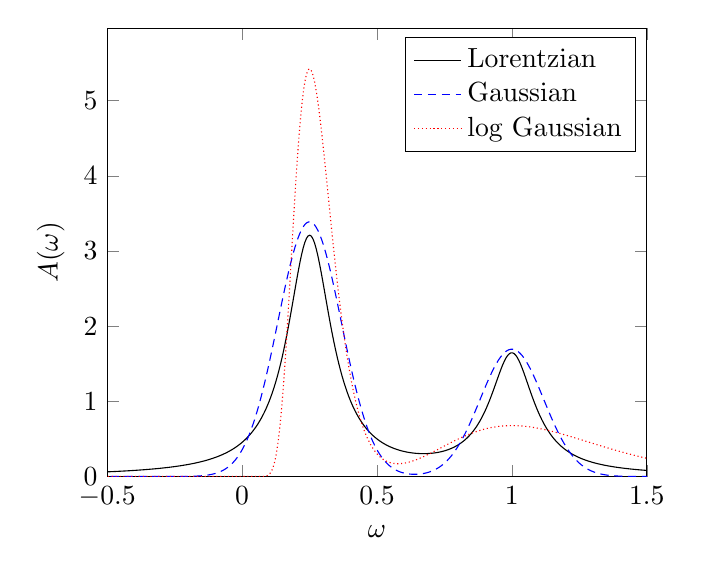
\begin{tikzpicture}
    \begin{axis}
        [
            xlabel=$\omega$,
            ylabel=$A(\omega)$,
            xmin=-0.5,
            xmax=1.5,
            ymin=0,
            legend cell align=left,
        ]

        % weight and locations of two poles
        \def\L{0.25}
        \def\W{1.0}
        \def\LL{1.0}
        \def\WW{0.5}

        % Lorentzian
        \def\DELTA{0.1}
        \addplot [color=black, domain=-1:2, samples=500] { \DELTA/pi*(\W/((x-\L)^2 + \DELTA^2) + \WW/((x-\LL)^2 + \DELTA^2))};
        \addlegendentry{Lorentzian}

        % Gaussian
        \def\SIGMA{0.11774100225154747} % HWHM sqrt(2*ln(2))*\DELTA
        \addplot [color=blue, densely dashed, domain=-1:2, samples=500] { 1/sqrt(2*pi*\SIGMA^2)*(\W*exp(-(x-\L)^2 / 2/ \SIGMA^2) + \WW*exp(-(x-\LL)^2 / 2 / \SIGMA^2))};
        \addlegendentry{Gaussian}

        % logarithmic Gaussian
        \def\B{0.4}
        \addplot [color=red, densely dotted, domain=-1:2, samples=900] { x > 0 ? exp(-\B^2 / 4) / (\B*sqrt(pi)) * (\W / \L *exp(-ln(x/\L)^2 / \B^2) + \WW / \LL *exp(-ln(x/\LL)^2 / \B^2)) : 0 };
        \addlegendentry{log Gaussian}
    \end{axis}
\end{tikzpicture}

    \caption{
        Spectral part of a correlator
        $C_\omega = \frac{1}{\omega + \mi0^+ - 0.25} + \frac{0.5}{\omega + \mi0^+ - 1}$
        using various broadening schemes.
    }%
    \label{fig:broadening}
\end{figure}

A comparison of these broadenings is given in \zcref{fig:broadening}.
The Lorentzian and Gaussian spectra consist of symmetric peaks
with the former decaying slower compared to the latter.
The peaks generated by the logarithmic Gaussian are asymmetric
and sharper if the pole is closer to $\omega=0$.
As all poles are at located at $\omega>0$,
the spectrum of the log Gaussian vanishes for $\omega\le0$.

\subsection{Self-energy}

In~\cite{Lu2014},
this equation was used to represent the self-energy by the constant Hartree term $\Sigma^\mH$
and a sum of poles
\begin{equation}
    \Sigma_\omega = \Sigma^\mH + \sum_j \frac{w_j}{\omega + \mi0^+ - \epsilon_j}.
    \label{eq:self-energy-sum-of-poles}
\end{equation}
For the self-energy to be physical, all weights must be positive.
On a system with finite bath sites and floating-point arithmetic however,
this was violated and poles with negative weight had to be merged into neighbors
such that only positive weight remained.

Given each correlator as a sum of poles,~\citeauthor{Kugler2022}~\cite{Kugler2022} broadened
each correlator and calculated the broadened self-energy $\Sigma_z$.
In this work we instead calculate the self-energy on the real axis
using the Schur complement~\cite{Schur1917}
\fe{TODO:\@ credit Aleksandrs} %TODO: credit Aleksandrs
\begin{equation}
    \Sigma_\omega = \Sigma^\mH + \left([(C_\omega)^{-1}]_{11}\right)^{-1}.
\end{equation}
To invert our block correlation function, we first bring it to
the Anderson representation (\zcref{eq:correlator-anderson}):
\begin{equation}
    C_\omega = B\frac{1}{\omega + \mi0^+ - A - D_\omega}B,
\end{equation}
with matrices $A$, $B$ and a block sum of poles $D_\omega$.
The scaling matrix $B$ contains the square root of the zeroth moments,
e.g.\ its first element $B_{11} = U/2$ at half-filling.
Due to the quadratic shift (\zcref{eq:quadratic-shift}), it is diagonal.
The Schur complement is then
\begin{equation}
    \left([(C_\omega)^{-1}]_{11}\right)^{-1}
    =
    B_{11} \frac{1}{\omega + \mi0^+ - A_{11} - (D_\omega)_{11}} B_{11}.
\end{equation}
Diagonalizing this expression gives us the self-energy in the same form as
\zcref{eq:self-energy-sum-of-poles}.
Contrasting against \zcref{eq:Dyson},
all pole weights are positive by construction
and no merging of negative weight into neighbors is necessary.
